\documentclass{article}
\iffalse
This file is protected by Copyright. Please refer to the COPYRIGHT file
distributed with this source distribution.

This file is part of OpenCPI <http://www.opencpi.org>

OpenCPI is free software: you can redistribute it and/or modify it under the
terms of the GNU Lesser General Public License as published by the Free Software
Foundation, either version 3 of the License, or (at your option) any later
version.

OpenCPI is distributed in the hope that it will be useful, but WITHOUT ANY
WARRANTY; without even the implied warranty of MERCHANTABILITY or FITNESS FOR A
PARTICULAR PURPOSE. See the GNU Lesser General Public License for more details.

You should have received a copy of the GNU Lesser General Public License along
with this program. If not, see <http://www.gnu.org/licenses/>.
\fi
\author{} % Force author to be blank
%----------------------------------------------------------------------------------------
% Paper size, orientation and margins
%----------------------------------------------------------------------------------------
\usepackage{geometry}
\geometry{
	letterpaper,			% paper type
	portrait,				% text direction
	left=.75in,				% left margin
	top=.75in,				% top margin
	right=.75in,			% right margin
	bottom=.75in			% bottom margin
 }
%----------------------------------------------------------------------------------------
% Header/Footer
%----------------------------------------------------------------------------------------
\usepackage{fancyhdr} \pagestyle{fancy} % required for fancy headers
\renewcommand{\headrulewidth}{0.5pt}
\renewcommand{\footrulewidth}{0.5pt}
\rhead{\small{ANGRYVIPER Team}}
%----------------------------------------------------------------------------------------
% Appendix packages
%----------------------------------------------------------------------------------------
\usepackage[toc,page]{appendix}
%----------------------------------------------------------------------------------------
% Defined Commands & Renamed Commands
%----------------------------------------------------------------------------------------
\renewcommand{\contentsname}{Table of Contents}
\renewcommand{\listfigurename}{List of Figures}
\renewcommand{\listtablename}{List of Tables}
\newcommand{\todo}[1]{\textcolor{red}{TODO: #1}\PackageWarning{TODO:}{#1}} % To do notes
\newcommand{\code}[1]{\texttt{#1}} % For inline code snippet or command line
%----------------------------------------------------------------------------------------
% Various pacakges
%----------------------------------------------------------------------------------------
\usepackage{hyperref} % for linking urls and lists
\usepackage{graphicx} % for including pictures by file
\usepackage{listings} % for coding language styles
\usepackage{rotating} % for sideways table
\usepackage{pifont}   % for sideways table
\usepackage{pdflscape} % for landscape view
%----------------------------------------------------------------------------------------
% Table packages
%----------------------------------------------------------------------------------------
\usepackage{tabularx} % c=center,l=left,r=right,X=fill
\usepackage{float}
\floatstyle{plaintop}
\usepackage[tableposition=top]{caption}
\newcolumntype{P}[1]{>{\centering\arraybackslash}p{#1}}
\newcolumntype{M}[1]{>{\centering\arraybackslash}m{#1}}
%----------------------------------------------------------------------------------------
% Block Diagram / FSM Drawings
%----------------------------------------------------------------------------------------
\usepackage{tikz}
\usetikzlibrary{shapes,arrows,fit,positioning}
\usetikzlibrary{automata} % used for the fsm
%----------------------------------------------------------------------------------------
% Colors Used
%----------------------------------------------------------------------------------------
\usepackage{colortbl}
\definecolor{blue}{rgb}{.7,.8,.9}
\definecolor{ceruleanblue}{rgb}{0.16, 0.32, 0.75}
\definecolor{drkgreen}{rgb}{0,0.6,0}
\definecolor{deepmagenta}{rgb}{0.8, 0.0, 0.8}
\definecolor{cyan}{rgb}{0.0,0.6,0.6}
\definecolor{maroon}{rgb}{0.5,0,0}
%----------------------------------------------------------------------------------------
% Update the docTitle and docVersion per document
%----------------------------------------------------------------------------------------
\def\docTitle{Component Data Sheet}
\def\docVersion{1.3}
%----------------------------------------------------------------------------------------
\date{Version \docVersion} % Force date to be blank and override date with version
\title{\docTitle}
\lhead{\small{\docTitle}}
\graphicspath{ {figures/} }

\def\comp{file\_read}
\def\Comp{File\ Read }
\graphicspath{ {figures/} }

\begin{document}

\section*{Summary - \Comp}
\begin{tabular}{|c|M{13.5cm}|}
	\hline
	\rowcolor{blue}
	                  &                                                                                \\
	\hline
	Name              & \comp                                                                          \\
	\hline
	Worker Type       & Application                                                                    \\
	\hline
	Version           &  v\docVersion \\
	\hline
	Release Date      &  September 2018 \\
	\hline
	Component Library &   ocpi.core\\
	\hline
	Workers           &  file\_read.rcc file\_read.hdl\\
	\hline
	Tested Platforms  &  isim, xsim, modelsim, xilinx13\_3, xilinx13\_4, centos6, centos7\\
	\hline
\end{tabular}

\section*{Functionality}
\begin{flushleft}
The File\_Read component injects file-based data into an application. It is used
by specifying an instance of the File\_Read component, and connecting its output port to
an input port of the component which will process the data first. The name of the file to
be read is specified in a property.
\subsection*{Operating Modes}
\subsubsection*{Data Streaming Mode}
In data streaming mode, the contents of the file becomes the payloads of a stream of
messages, each carrying a fixed number of bytes of file data and all with
the same opcode. The length and opcode of all output messages are specified as
properties. This means that this mode only lends itself to protocols that have a single opcode or the intent is to only send data on one of the opcodes of a multi-opcode protocol.\\ \medskip \medskip
If the number of bytes in the file is not an even multiple of the message size the
remaining bytes are sent in a final shorter message. The granularity of messages can
also be specified. This forces the message size to be a multiple of this value, and
forces truncation of the final message to be a multiple of this value.
\subsubsection*{Messaging Mode}
In messaging mode, the contents of the file are interpreted as a sequence of defined
messages, with an 8-byte header in the file itself preceding the payload for each message.
This header contains the length and opcode of the message, with the data contents of
the message following the header. The length can be zero, meaning that a message
will be sent with the indicated opcode, and the length of the message will be zero.\\
\medskip \medskip
The first 32-bit word of the header is interpreted as the message length in bytes, little-endian. The next 8-bit byte is the opcode of the message, followed by 3 padding bytes.
If the end of the file is encountered while reading a message header, or while reading
the header-specified length of the message payload, an error will be reported and the
component will terminate.  The following Messaging File Field Layout shows the layout of a file: 

\begin{figure}[ht]
	\centerline{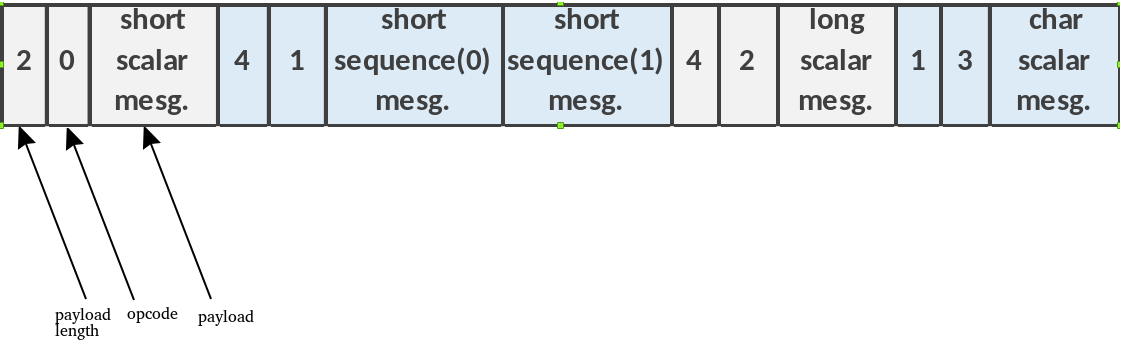
\includegraphics[scale=0.45]{MessageMode}}
	\caption{Messaging File Field Layout}
\end{figure}
\subsection*{No Protocol}
The port on the component has no protocol specified.  This means that the data file must be formatted to match the protocol of the input port of the connected worker.  For message mode this means only using opcodes and payloads in the file that correspond to the protocol of the connected component.  In data streaming mode the file structure needs to correspond to the opcode that is set by the \textit{opcode} property.
\subsection*{Message Size/Buffers}
The protocol of the connected component needs to be taken into account when selecting the message size (bytes) to prevent buffer overflow problems.  The component has no information about what component it is connected to (by design). The application designer needs to set a valid value.  For example iqstream protocol uses a sequence of 2048 16-bit I/Q pairs which means anything over 8192 (2048 * 4 bytes per pair) is invalid.
\subsection*{End of File Handling}
When the File\_Read component reaches the end of its input file, it will do one of three
things:
\begin{itemize}
  \item send a zero-length message (ZLM) with an opcode set by the \textit{opcode} property (default).  See Zero Length Messages section.
  \item enter the ``done'' state with no further action, when the \textit{suppressEOF} property
is true
  \item restart reading at the beginning of the file, when the \textit{repeat} property is true
\end{itemize}
\subsubsection*{Zero Length Messages}
A zero-length message (ZLM) is any message that has zero payload (data) associated with it but the rest of the message signaling and opcode are passed through.  The default operation for end-of-file for File\_Read is to pass along a ZLM on the opcode set by the property \textit{opcode} (default is 0) which is then advanced to the downstream worker. The ZLM is processed by the File\_Write component at the end of the application chain and File\_Write sets its state to``done''.  In file based applications it is common practice to set an application to complete when the File write component is done to ensure all data is processed.  This means that all other workers in the path must process and pass on ZLMs for this to function properly.

\end{flushleft}

\section*{Worker Implementation Details}
\subsection*{\comp.hdl}
\begin{flushleft}
This worker will only run on simulator platforms.  This includes isim, xsim, and modelsim and will not run on or be built for any other hardware platforms.  This is because it conatins code that cannot be realized into RTL.
\end{flushleft}
\subsection*{\comp.rcc}
\begin{flushleft}
This worker in implemented in the C language version of the RCC model.  Most new workers are implemented in the C++ language version of the RCC model.
\end{flushleft}

\section*{Source Dependencies}
\subsection*{\comp.rcc}
\begin{itemize}
\item file\_read.c
\item file\_read.h
\end{itemize}
\subsection*{\comp.hdl}
\begin{itemize}
\item file\_read.vhd
\end{itemize}


\begin{landscape}
	\section*{Component Spec Properties}
	\begin{scriptsize}
\begin{tabular}{|p{2cm}|p{2cm}|c|c|c|p{1.5cm}|p{1cm}|p{7cm}|}
\hline
\rowcolor{blue}
Name                 & Type   & SequenceLength & ArrayDimensions & Accessibility       & Valid Range & Default & Usage
\\
\hline
fileName & string length:1024 & - & - & Initial & -  &- & The name of the file whose contents are sent out as raw data to the output port.
\\
\hline
messagesInFile & bool  & - & - & Readable, Initial & -  &false & The flag that is used to turn on and off message mode. See section on Message Mode.
\\
\hline
opcode & uchar  & - & - & Readable, Initial & -  &0 & The Opcode that all the data in the datafile is sent in streaming mode. The opcode of the ZLM at the end of the file in messaging mode.
\\
\hline
messageSize & ulong  & - & - & Readable, Initial & -  &4096 & The size of the messages in bytes that are created on the output port.  The connected worker's buffer needs to be big enough to take the data buffer that is being passed to the worker.  See Output Port section.
\\
\hline
granularity & ulong  & - & - & Readable, Initial & -  &1 & The final message at the end of a file will truncated to be a multiple of this property's value in bytes.
\\
\hline
repeat & bool  & - & - & Writeable & -  &- & The flag used to repeat the data file over and over.
\\
\hline
bytesRead & uLongLong  & - & - & Volatile & -  &- & The number of bytes read from file.  Useful for debugging data flow issues.
\\
\hline
messagesWritten & uLongLong  & - & - & Volatile & -  &- & The number of messages read from file.  Good property for debugging data flow issues.
\\
\hline
suppressEOF & bool  & - & - & Initial & -  &- & The flag used to enable or disable the Zero Length message that is propagated at the end of the file.
\\
\hline
badMessage & bool  & - & - & Volatile & -  &- & This flag is set by the worker if the worker has a problem getting data from file. An example of this happening is a bad filename.
\\
\hline
\end{tabular}
	\end{scriptsize}

	\section*{Worker Properties}
	\subsection*{\comp.hdl}
	\begin{scriptsize}
\begin{tabular}{|p{2cm}|p{2.75cm}|p{3.5cm}|p{2cm}|p{2cm}|p{2.25cm}|p{1.5cm}|p{1cm}|p{4cm}|}
			\hline
			\rowcolor{blue}
			Type     & Name                      & Type  & SequenceLength & ArrayDimensions & Accessibility       & Valid Range & Default & Usage                                      \\
			\hline
			Spec Property & fileName & string  & - & - & Readable & -  &- & added Readable
            \\
            \hline
            Spec Property & suppressEOF & bool  & - & - & Readable & -  &- & added Readable
            \\
            \hline
            Property & CWD\_MAX\_LENGTH & ulong  & - & - & Paramater & -  & 256 & parameter for max string length for the cwd property
            \\
            \hline
            Property & cwd & string length:CWD\_MAX\_LENGTH & - & - & Volatile & -  &- & the current working direactory of the application (this is required for the hdl version of this worker and cannot be detiermined automaticly)
            \\
            \hline
    \end{tabular}
	\end{scriptsize}

	\subsection*{\comp.rcc}
    \begin{scriptsize}
    \begin{tabular}{|p{2cm}|p{2.75cm}|p{1cm}|p{2.75cm}|p{2cm}|p{2.25cm}|p{2cm}|p{1cm}|p{5cm}|}
			\hline
			\rowcolor{blue}
			Type     & Name                      & Type  & SequenceLength & ArrayDimensions & Accessibility       & Valid Range & Default & Usage                                      \\
			\hline
			Spec Property & fileName & string  & - & - & Readable & -  &- & added Readable
            \\
            \hline
            Spec Property & suppressEOF & bool  & - & - & Readable & -  &- & added Readable
            \\
            \hline
            Spec Property & messageSize & ulong  & - & - &  Volatile & -  &4096 & added Volatile
            \\
            \hline
    \end{tabular}
	\end{scriptsize}

	\section*{Component Ports}
	\begin{scriptsize}
\begin{tabular}{|M{2cm}|M{1.5cm}|M{4cm}|c|c|M{9cm}|}
\hline
\rowcolor{blue}
Name & Producer & Protocol & Optional & Advanced & Usage
\\
\hline
out & true & None& False & - & Data streamed from file\\
\hline
\end{tabular}
	\end{scriptsize}

	\section*{Worker Interfaces}
	\subsection*{\comp.hdl}
	\begin{scriptsize}
\begin{tabular}{|M{2cm}|M{1.5cm}|M{4cm}|c|M{12cm}|}
\hline
\rowcolor{blue}
Type & Name & DataWidth & Advanced & Usage
\\
\hline
StreamInterface & out & 32 & - & Data streamed from file\\
\hline
\end{tabular}
	\end{scriptsize}
\end{landscape}

\section*{Test and Verification}
\begin{flushleft}
All test benches use this worker as part of the verification process. A unit-test does not exist for this component.
\end{flushleft}
\end{document}
